
\special{dvipdfmx:config z 0} %取消PDF压缩,加快速度,最终版本生成的时候最好把这句话注释掉

\documentclass[11pt,a4paper,UTF8]{book}

\usepackage{verbatim}
\usepackage[T1]{fontenc}
\usepackage[utf8]{inputenc}
\usepackage{authblk}

\usepackage{fontspec}                  %引入字体设置宏包
\setmainfont{Times New Roman}             %设置英文正文字体
% Courier New
% Book Antique
\setsansfont{Arial}                    %英文无衬线字体
\setmonofont{Courier New}              %英文等宽字体

\usepackage{ctex} %导入中文包
%\usepackage{ulem}
\usepackage{tocvsec2}


\usepackage{tabularx}
\usepackage{longtable}
\usepackage{booktabs}
\usepackage{multirow}
\usepackage{bbding}
\usepackage{float}
\usepackage{xspace}
\usepackage[none]{hyphenat}
\usepackage{pgffor}

\usepackage{graphicx}
\usepackage{subfigure}
\usepackage{pifont}

\usepackage{hyperref}  %制作pdf的目录
\usepackage{subfiles} %使用多文件方式进行

\usepackage{geometry} %设置页边距的包
\geometry{left=2.5cm,right=2cm,top=2.54cm,bottom=2.54cm} %设置书籍的页边距

\usepackage{url}
\hypersetup{hidelinks, %去红框
  colorlinks=true,
  allcolors=black,
  pdfstartview=Fit,
  breaklinks=true
}

% 调整itemlist中的行间距
\usepackage{enumitem}
\setenumerate[1]{itemsep=0pt,partopsep=0pt,parsep=\parskip,topsep=5pt}
\setitemize[1]{itemsep=0pt,partopsep=0pt,parsep=\parskip,topsep=5pt}
\setdescription{itemsep=0pt,partopsep=0pt,parsep=\parskip,topsep=5pt}

% 超链接样式设置
\usepackage{hyperref}
\hypersetup{
  colorlinks=true,
  linkcolor=blue,
  filecolor=blue,
  urlcolor=blue,
  citecolor=cyan,
}

\usepackage{indentfirst}

\usepackage{listings}
\usepackage[usenames,dvipsnames,svgnames, x11names]{xcolor}
\usepackage{wallpaper}

\usepackage[most]{tcolorbox}
\tcbuselibrary{breakable, minted, skins}

%https://tex.stackexchange.com/questions/173850/problem-in-adding-a-background-color-in-a-minted-environment
\newtcblisting{shell}{
    listing engine=minted,
    minted language=text,%bash, % 使用text就不会有语法高亮显示
    minted options={autogobble,linenos,breaklines},
    listing only,
    size=title,
    arc=0.3mm,
    breakable,
    enhanced jigsaw,
    colframe=black!50!white,
    boxrule=0.5mm,
    colback=bashcodebg,
    coltext=Black,
    minted options={linenos=false,texcl=true},
}
\definecolor{bashcodebg}{rgb}{0.85,0.85,0.85}

% https://tex.stackexchange.com/questions/304449/combine-minted-and-tcolorbox-for-code-from-file-inputminted
\newcounter{inputPrg}
\newtcblisting[use counter=inputPrg, number format=\arabic]{cpp}{
    listing engine=minted,
    minted language=c++,
    minted options={autogobble,linenos,breaklines},
    listing only,
    size=title,
    arc=0.5mm,
    breakable,
    enhanced jigsaw,
    colframe=black!7!white,
    %coltitle=White,
    boxrule=0.5mm,
    colback=blue!3!white,
    coltext=Black,
    %title=\TwoSymbolsAndText{\faCode}{%
        %    \textbf{Input program \thetcbcounter}\ifthenelse{\equal{#2}{}}{}{\textbf{:} \textit{#2}}%
        %}{\faCode},
    %label=inputPrg:#3
    left=6.5mm,enhanced,
    overlay={\begin{tcbclipinterior}\fill[black!5] (frame.south west)
            rectangle ([xshift=5mm]frame.north west);\end{tcbclipinterior}}
}

\usepackage{tikz}

% URL 正确换行
% https://liam.page/2017/05/17/help-the-url-command-from-hyperref-to-break-at-line-wrapping-point/
\makeatletter
\def\UrlAlphabet{%
  \do\a\do\b\do\c\do\d\do\e\do\f\do\g\do\h\do\i\do\j%
  \do\k\do\l\do\m\do\n\do\o\do\p\do\q\do\r\do\s\do\t%
  \do\u\do\v\do\w\do\x\do\y\do\z\do\A\do\B\do\C\do\D%
  \do\E\do\F\do\G\do\H\do\I\do\J\do\K\do\L\do\M\do\N%
  \do\O\do\P\do\Q\do\R\do\S\do\T\do\U\do\V\do\W\do\X%
  \do\Y\do\Z}
\def\UrlDigits{\do\1\do\2\do\3\do\4\do\5\do\6\do\7\do\8\do\9\do\0}
\g@addto@macro{\UrlBreaks}{\UrlOrds}
\g@addto@macro{\UrlBreaks}{\UrlAlphabet}
\g@addto@macro{\UrlBreaks}{\UrlDigits}
\makeatother

% enable subsubsubsection
% from https://tex.stackexchange.com/练习题/274212/correct-hierarchy-levels-of-pdf-bookmarks-for-custom-section-subsubsubsection
\usepackage[depth=3]{bookmark}
\setcounter{secnumdepth}{3}
\setcounter{tocdepth}{4}
\hypersetup{bookmarksdepth=4}

\makeatletter

\newcommand{\toclevel@subsubsubsection}{4}
\newcounter{subsubsubsection}[subsubsection]

\renewcommand{\thesubsubsubsection}{\thesubsubsection.\arabic{subsubsubsection}}

\newcommand{\subsubsubsection}{\@startsection{subsubsubsection}{4}{\z@}%
  {-3.25ex\@plus -1ex \@minus -.2ex}%
  {1.5ex \@plus .2ex}%
  {\normalfont\normalsize\bf\bfseries}}

\newcommand*{\l@subsubsubsection}{\@dottedtocline{4}{11em}{5em}}

\newcommand{\subsubsubsectionmark}[1]{}
\makeatother


\ExplSyntaxOn

% Setup enumerate, itemize and description
\setenumerate  { nosep }
\setitemize    { nosep }
\setdescription{ nosep }

% Setup minted
\setminted { obeytabs, tabsize=2, breaklines=true, fontsize=\footnotesize}

% Def \filename
\NewDocumentCommand { \filename } { m }
{ \noindent  \hspace*{\fill} \\ \textit { #1 } \vspace*{ -1ex } \nopagebreak[4] }

% Def \mySamllsection
\NewDocumentCommand { \mySamllsection } { m }
{\vspace{ 0.2cm } \noindent \textbf { #1 } \vspace*{ 0.05cm } \nopagebreak[4] }

\NewDocumentCommand { \myGraphic } { mmm }
{
  \begin{center}
    \includegraphics[width={#1}\textwidth]{#2}\\
    {#3}
  \end{center}
}

% Def \inlcpp
\NewDocumentCommand { \inlcpp }   { m }
{ \mintinline { cpp } { #1 } }

% Def cpp environment
%\NewDocumentEnvironment { cpp } { }
%{ \VerbatimEnvironment
%  \begin { minted } [ linenos=true, frame=single ] { cpp } }
%{ \end   { minted } }

% Def cmake environment
\NewDocumentEnvironment { cmake } { }
{ \VerbatimEnvironment
  \begin { minted } [ linenos=true, frame=single ] { cmake } }
{ \end   { minted } }

\NewDocumentEnvironment { myNotic } { m }
{ %\hspace*{\fill} \\
  \begin { tcolorbox } [ breakable,colback = blue!5!white, colframe=blue!55!black ,title={#1}] }
{ \end   { tcolorbox } }

\NewDocumentEnvironment { myTip } { m }
{ %\hspace*{\fill} \\
  \begin { tcolorbox } [ breakable,colback = green!5!white, colframe=green!45!black ,title={#1}] }
{ \end   { tcolorbox } }

\NewDocumentEnvironment { myWarning } { m }
{ %\hspace*{\fill} \\
  \begin { tcolorbox } [ breakable,colback=red!5!white,colframe=red!55!black,title={#1}] }
{ \end   { tcolorbox } }

\NewDocumentCommand { \mySubsubsection } { mm }
{
\subsubsection*{\zihao{3} {#1} \hspace{0.2cm}{#2}}
\addcontentsline{toc}{subsubsection}{{#1}\hspace{0.2cm}{#2}}
}

\NewDocumentCommand { \mySubsectionNoFile } { mm }
{
\subsection*{\zihao{3}{#1}\hspace{0.2cm}{#2}}
\addcontentsline{toc}{subsection}{{#1}\hspace{0.2cm}{#2}}
}

\NewDocumentCommand { \mySubsection } { mmm }
{
\subsection*{\zihao{3}{#1}\hspace{0.2cm}{#2}}
\addcontentsline{toc}{subsection}{{#1}\hspace{0.2cm}{#2}}
\subfile{{#3}}
}

\NewDocumentCommand { \mySectionNoHeadImage } { mmm }
{
\color{black}
\pagecolor{white}
\section*{\zihao{2}{#1}\hspace{0.5cm}{#2}}
\addcontentsline{toc}{section}{{#1}\hspace{0.5cm}{#2}}
\subfile{{#3}}
}

\NewDocumentCommand { \mySection } { mmm }
{
%\ThisULCornerWallPaper{1.0}{images/section-header.png}
\section*{\zihao{2}{#1}\hspace{0.5cm}{#2}}
\addcontentsline{toc}{section}{{#1}\hspace{0.5cm}{#2}}
\subfile{{#3}}
}

\NewDocumentCommand { \myPart } { mmm }
{
%\ThisCenterWallPaper{1.15}{images/section-background.png}
\section*{\zihao{2}{#1}\hspace{0.5cm}{#2}}
\addcontentsline{toc}{section}{{#1}\hspace{0.5cm}{#2}}
\subfile{{#3}}
}

% Latex如何在文本模式批量处理下划线
% https://zhuanlan.zhihu.com/p/615108006

\ExplSyntaxOff

\begin{document}
\begin{sloppypar} %latex中一行文字出现溢出问题的解决方法
%\maketitle

\begin{center}
\thispagestyle{empty}
%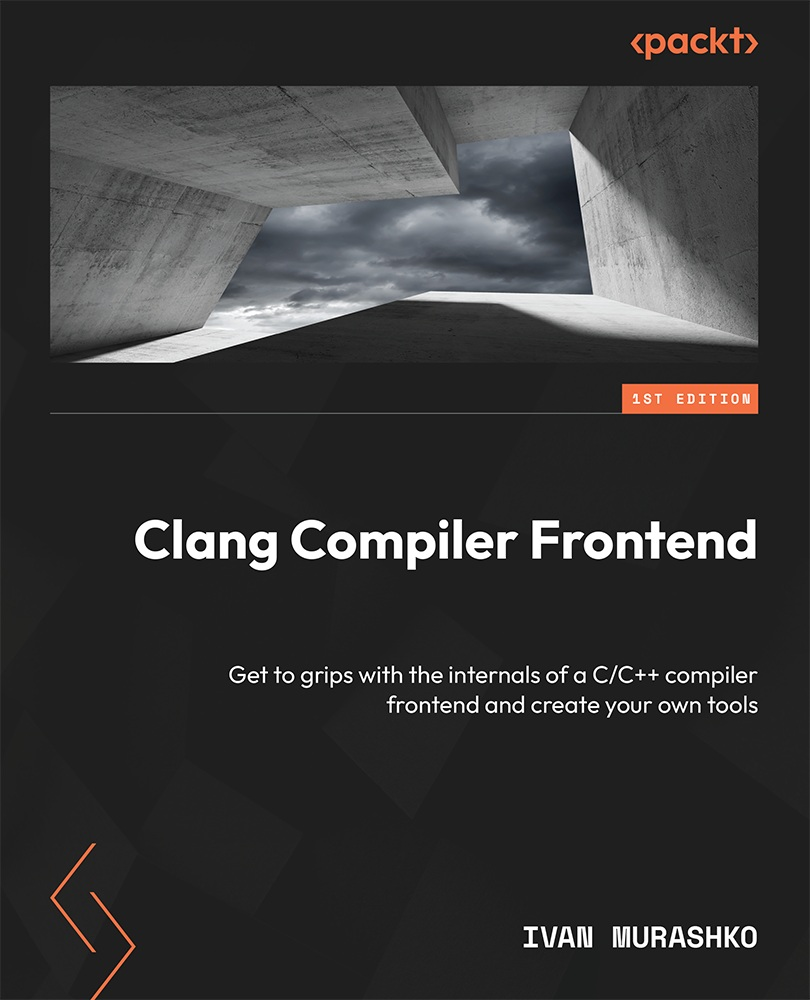
\includegraphics[width=\textwidth,height=\textheight,keepaspectratio]{cover.png}
\begin{tikzpicture}[remember picture, overlay, inner sep=0pt]
\node at (current page.center)
{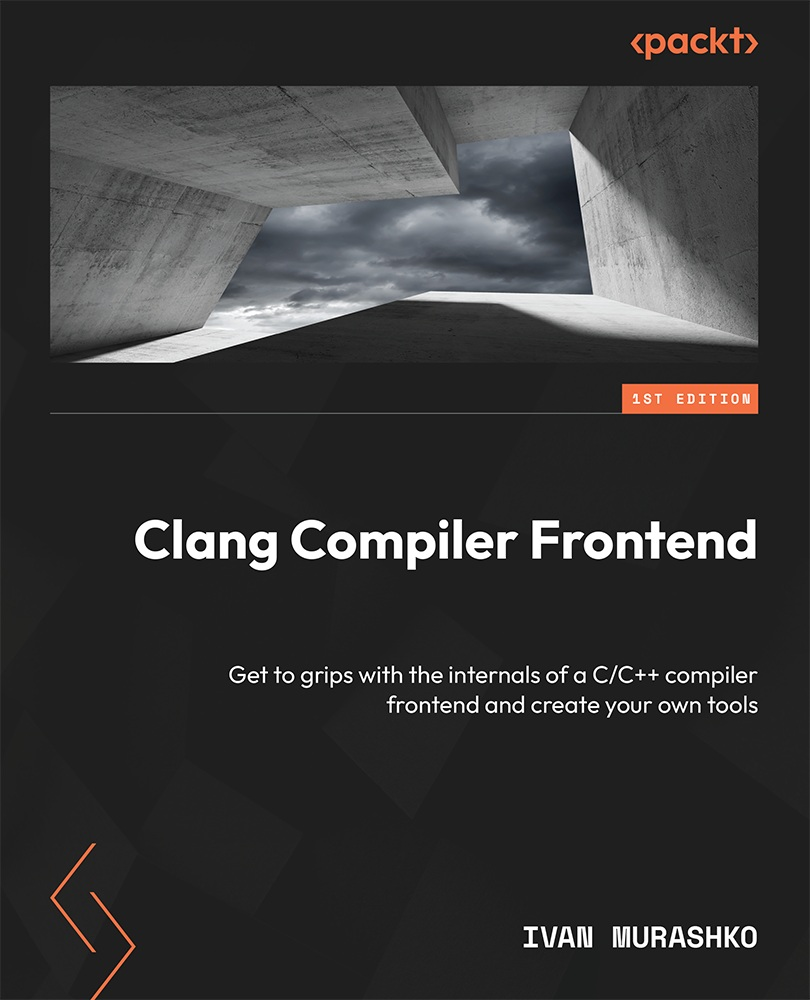
\includegraphics[width=\paperwidth, keepaspectratio=false]{cover.png}};
\end{tikzpicture}
\newpage
\thispagestyle{empty}
\huge
\textbf{Clang Compiler Frontend}
\\[9pt]
{\Large Get to grips with the internals of a C/C++ compiler frontend and create your own tools}
\\[9pt]
\normalsize
作者: Ivan Murashko
\\[8pt]
\normalsize
译者:\href{https://github.com/xiaoweiChen/Clang-Compiler-Frontend}{陈晓伟}
\\[8pt]
\end{center}

\newpage

\begin{comment}
\end{comment}
\pagestyle{empty}
\tableofcontents
\newpage

\setsecnumdepth{section}

\mySectionNoHeadImage{}{关于作者}{content/about-the-author.tex}
\newpage

\mySectionNoHeadImage{}{关于评审}{content/about-the-reviewer.tex}
\newpage

\mySectionNoHeadImage{}{前言}{content/preface.tex}
\newpage

\myPart{第一部分}{Clang Setup and Architecture}{content/part1/title.tex}
\newpage

\mySection{第1章}{Environment Setup}{content/part1/chapter1/0.tex}
\mySubsection{1.1.}{Technical requirements}{content/part1/chapter1/1.tex}
\mySubsection{1.2.}{Getting to know LLVM}{content/part1/chapter1/2.tex}
\mySubsection{1.3.}{Source code compilation}{content/part1/chapter1/3.tex}
\mySubsection{1.4.}{Test project - syntax check with a Clang tool}{content/part1/chapter1/4.tex}
\mySubsection{1.5.}{总结}{content/part1/chapter1/5.tex}
\mySubsection{1.6.}{扩展阅读}{content/part1/chapter1/6.tex}
\newpage

\mySection{第2章}{Clang Architecture}{content/part1/chapter2/0.tex}
\mySubsection{2.1.}{Technical requirements}{content/part1/chapter2/1.tex}
\mySubsection{2.2.}{Getting started with compilers}{content/part1/chapter2/2.tex}
\mySubsection{2.3.}{Clang driver overview}{content/part1/chapter2/3.tex}
\mySubsection{2.4.}{Clang fronted overview}{content/part1/chapter2/4.tex}
\mySubsection{2.5.}{总结}{content/part1/chapter2/5.tex}
\mySubsection{2.6.}{扩展阅读}{content/part1/chapter2/6.tex}
\newpage

\mySection{第3章}{Clang AST}{content/part1/chapter3/0.tex}
\mySubsection{3.1.}{Technical requirements}{content/part1/chapter3/1.tex}
\mySubsection{3.2.}{AST}{content/part1/chapter3/2.tex}
\mySubsection{3.3.}{AST traversal}{content/part1/chapter3/3.tex}
\mySubsection{3.4.}{Recursive AST visitor}{content/part1/chapter3/4.tex}
\mySubsection{3.5.}{AST matchers}{content/part1/chapter3/5.tex}
\mySubsection{3.6.}{Explore Clang AST with clang-query}{content/part1/chapter3/6.tex}
\mySubsection{3.7.}{Processing Ast in the case of errors}{content/part1/chapter3/7.tex}
\mySubsection{3.8.}{总结}{content/part1/chapter3/8.tex}
\mySubsection{3.9.}{扩展阅读}{content/part1/chapter3/9.tex}
\newpage

\mySection{第4章}{Basic Libraries and Tools}{content/part1/chapter4/0.tex}
\mySubsection{4.1.}{Technical requirements}{content/part1/chapter4/1.tex}
\mySubsection{4.2.}{LLVM coding style}{content/part1/chapter4/2.tex}
\mySubsection{4.3.}{LLVM basic libraries}{content/part1/chapter4/3.tex}
\mySubsection{4.4.}{Clang basic libraries}{content/part1/chapter4/4.tex}
\mySubsection{4.5.}{LLVM supporting tools}{content/part1/chapter4/5.tex}
\mySubsection{4.6.}{Clang plugin project}{content/part1/chapter4/6.tex}
\mySubsection{4.7.}{总结}{content/part1/chapter4/7.tex}
\mySubsection{4.8.}{扩展阅读}{content/part1/chapter4/8.tex}
\newpage

\myPart{第二部分}{Clang Tools}{content/part2/title.tex}
\newpage

\mySection{第5章}{Clang-Tidy Linter Framework}{content/part2/chapter5/0.tex}
\mySubsection{5.1.}{Technical requirements}{content/part2/chapter5/1.tex}
\mySubsection{5.2.}{Overview of Clang-Tidy and usage examples}{content/part2/chapter5/2.tex}
\mySubsection{5.3.}{Clang-Tidy;s internal design}{content/part2/chapter5/3.tex}
\mySubsection{5.4.}{Custom Clang-Tidy check}{content/part2/chapter5/4.tex}
\mySubsection{5.5.}{总结}{content/part2/chapter5/5.tex}
\mySubsection{5.6.}{扩展阅读}{content/part2/chapter5/6.tex}
\newpage

\mySection{第6章}{Advanced Code Analysis}{content/part2/chapter6/0.tex}
\mySubsection{6.1.}{Technical requirements}{content/part2/chapter6/1.tex}
\mySubsection{6.2.}{Static analysis}{content/part2/chapter6/2.tex}
\mySubsection{6.3.}{CFG}{content/part2/chapter6/3.tex}
\mySubsection{6.4.}{Custom CFG check}{content/part2/chapter6/4.tex}
\mySubsection{6.5.}{CFG on Clang}{content/part2/chapter6/5.tex}
\mySubsection{6.6.}{Brief description of Clang analysis tools}{content/part2/chapter6/6.tex}
\mySubsection{6.7.}{Knowing the limitations of analysis}{content/part2/chapter6/7.tex}
\mySubsection{6.8.}{总结}{content/part2/chapter6/8.tex}
\mySubsection{6.9.}{扩展阅读}{content/part2/chapter6/9.tex}
\newpage

\mySection{第7章}{Refactoring Tools}{content/part2/chapter7/0.tex}
\mySubsection{7.1.}{Technical requirements}{content/part2/chapter7/1.tex}
\mySubsection{7.2.}{Custom code modification tool}{content/part2/chapter7/2.tex}
\mySubsection{7.3.}{Clang-Tidy as a code modification tool}{content/part2/chapter7/3.tex}
\mySubsection{7.4.}{Code modification and Clang-Format}{content/part2/chapter7/4.tex}
\mySubsection{7.5.}{总结}{content/part2/chapter7/5.tex}
\mySubsection{7.6.}{扩展阅读}{content/part2/chapter7/6.tex}
\newpage

\mySection{第8章}{IDE Support and Clangd}{content/part2/chapter8/0.tex}
\mySubsection{8.1.}{Technical requirements}{content/part2/chapter8/1.tex}
\mySubsection{8.2.}{Language Server Protocol}{content/part2/chapter8/2.tex}
\mySubsection{8.3.}{Environment setup}{content/part2/chapter8/3.tex}
\mySubsection{8.4.}{LSP demo}{content/part2/chapter8/4.tex}
\mySubsection{8.5.}{Integration with Clang tools}{content/part2/chapter8/5.tex}
\mySubsection{8.6.}{performance optimizations}{content/part2/chapter8/6.tex}
\mySubsection{8.7.}{总结}{content/part2/chapter8/7.tex}
\mySubsection{8.8.}{扩展阅读}{content/part2/chapter8/8.tex}
\newpage

\myPart{第三部分}{附录}{content/part3/title.tex}
\newpage

\mySection{附录A}{Compilation Database}{content/part3/appendix-A/0.tex}
\mySubsection{A.1.}{Compilation database definition}{content/part3/appendix-A/1.tex}
\mySubsection{A.2.}{CDB ceration}{content/part3/appendix-A/2.tex}
\mySubsection{A.3.}{Clang tools and a CDB}{content/part3/appendix-A/3.tex}
\mySubsection{A.4.}{扩展阅读}{content/part3/appendix-A/4.tex}
\newpage

\mySection{附录B}{Build Speed Optimization}{content/part3/appendix-B/0.tex}
\mySubsection{B.1.}{Technical requirements}{content/part3/appendix-B/1.tex}
\mySubsection{B.2.}{Precompiled headers}{content/part3/appendix-B/2.tex}
\mySubsection{B.3.}{Clang modules}{content/part3/appendix-B/3.tex}
\mySubsection{B.4.}{扩展阅读}{content/part3/appendix-B/4.tex}
\newpage

\mySection{附录C}{Bibliography}{content/part3/appendix-C/0.tex}
\newpage

\begin{comment}
\end{comment}

\end{sloppypar}
\end{document}

